\documentclass{standalone}
\usepackage{tikz}
\usetikzlibrary{patterns, positioning}
\usepackage[sfdefault]{ClearSans} %% option 'sfdefault' activates Clear Sans as the default text font
\usepackage[T1]{fontenc}

\begin{document}
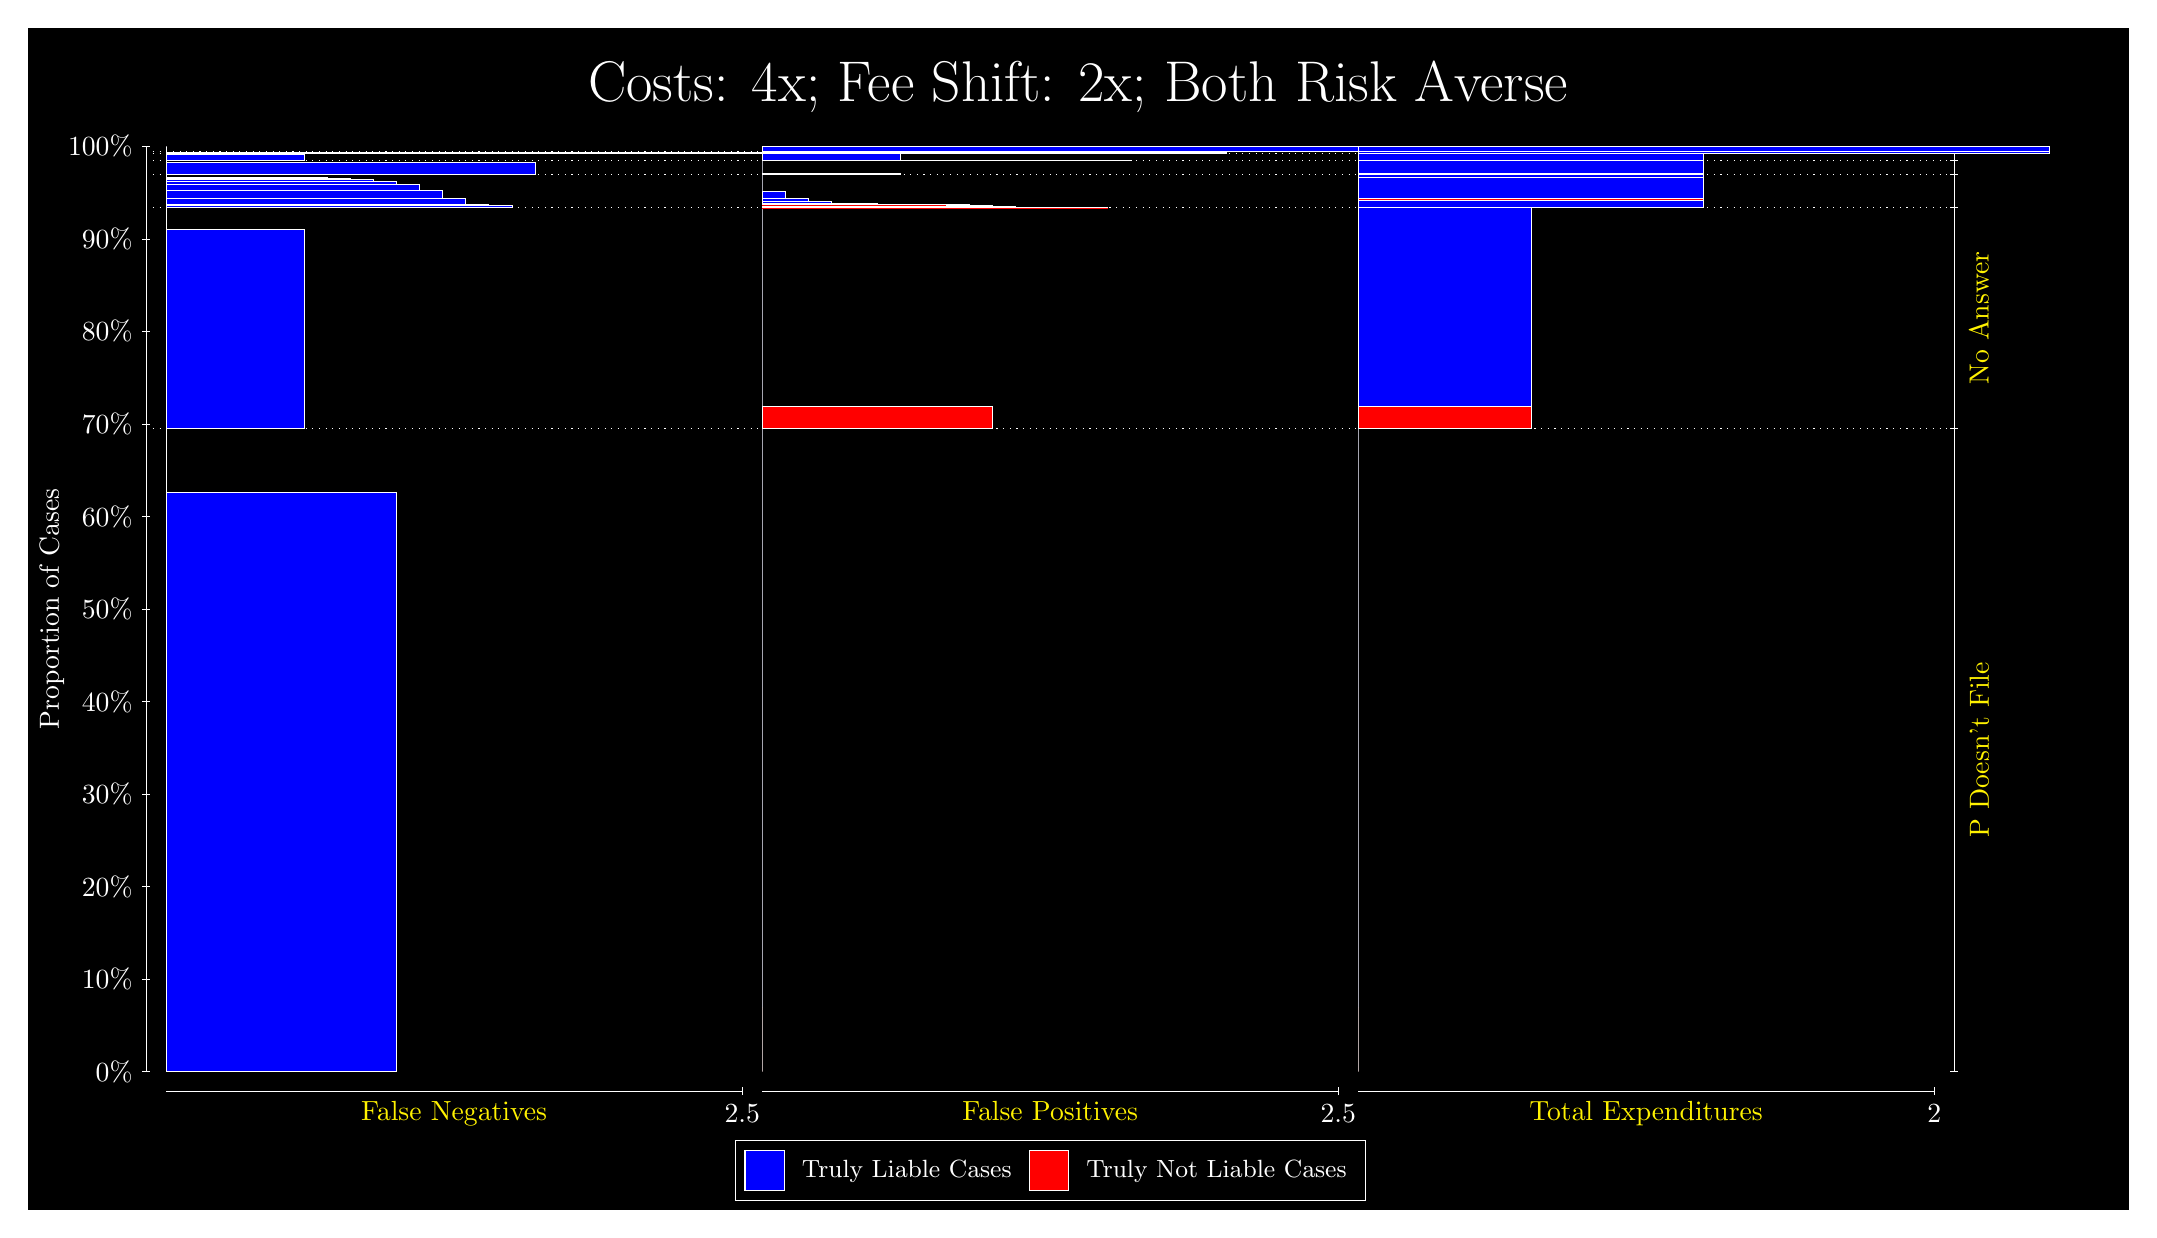
\begin{tikzpicture}
\draw[fill=black] (0,0) rectangle (26.667,15);
\draw[text=white] (0,13.5) rectangle (26.667,15) node[midway] {\huge Costs: 4x; Fee Shift: 2x; Both Risk Averse};
\draw[white, very thin] (1.5,1.75) -- (1.5,13.5);
\node[rotate=90, text=white, anchor=center] at (0.3, 7.625) {Proportion of Cases};
\draw[white, very thin] (1.45,1.75) -- (1.55,1.75);
\node[text=white, anchor=east] at (1.45, 1.75) {0\%};
\draw[white, very thin] (1.45,2.925) -- (1.55,2.925);
\node[text=white, anchor=east] at (1.45, 2.925) {10\%};
\draw[white, very thin] (1.45,4.1) -- (1.55,4.1);
\node[text=white, anchor=east] at (1.45, 4.1) {20\%};
\draw[white, very thin] (1.45,5.275) -- (1.55,5.275);
\node[text=white, anchor=east] at (1.45, 5.275) {30\%};
\draw[white, very thin] (1.45,6.45) -- (1.55,6.45);
\node[text=white, anchor=east] at (1.45, 6.45) {40\%};
\draw[white, very thin] (1.45,7.625) -- (1.55,7.625);
\node[text=white, anchor=east] at (1.45, 7.625) {50\%};
\draw[white, very thin] (1.45,8.8) -- (1.55,8.8);
\node[text=white, anchor=east] at (1.45, 8.8) {60\%};
\draw[white, very thin] (1.45,9.975) -- (1.55,9.975);
\node[text=white, anchor=east] at (1.45, 9.975) {70\%};
\draw[white, very thin] (1.45,11.15) -- (1.55,11.15);
\node[text=white, anchor=east] at (1.45, 11.15) {80\%};
\draw[white, very thin] (1.45,12.325) -- (1.55,12.325);
\node[text=white, anchor=east] at (1.45, 12.325) {90\%};
\draw[white, very thin] (1.45,13.5) -- (1.55,13.5);
\node[text=white, anchor=east] at (1.45, 13.5) {100\%};

\draw[white, very thin] (24.457,1.75) -- (24.457,13.5);
\draw[white, very thin] (24.407,1.75) -- (24.507,1.75);
\node[anchor=west] at (24.407, 1.75) {};
\draw[white, very thin] (24.407,9.9169) -- (24.507,9.9169);
\node[anchor=west] at (24.407, 9.9169) {};
\draw[white, very thin] (24.407,12.721) -- (24.507,12.721);
\node[anchor=west] at (24.407, 12.721) {};
\draw[white, very thin] (24.407,13.143) -- (24.507,13.143);
\node[anchor=west] at (24.407, 13.143) {};
\draw[white, very thin] (24.407,13.318) -- (24.507,13.318);
\node[anchor=west] at (24.407, 13.318) {};
\draw[white, very thin] (24.407,13.41) -- (24.507,13.41);
\node[anchor=west] at (24.407, 13.41) {};
\draw[white, very thin] (24.407,13.436) -- (24.507,13.436);
\node[anchor=west] at (24.407, 13.436) {};
\draw[white, very thin] (24.407,13.5) -- (24.507,13.5);
\node[anchor=west] at (24.407, 13.5) {};

\draw[white, very thin, fill=blue] (1.75,1.75) rectangle (4.6775,9.1002);
\draw[white, very thin, fill=red] (1.75,9.1002) rectangle (1.75,9.9169);
\draw[white, very thin, fill=blue] (1.75,9.9169) rectangle (3.5065,12.443);
\draw[white, very thin, fill=red] (1.75,12.443) rectangle (1.75,12.721);
\draw[white, very thin, fill=blue] (1.75,12.721) rectangle (6.1413,12.75);
\draw[white, very thin, fill=blue] (1.75,12.75) rectangle (5.8486,12.768);
\draw[white, very thin, fill=blue] (1.75,12.768) rectangle (5.5558,12.846);
\draw[white, very thin, fill=blue] (1.75,12.846) rectangle (5.2631,12.938);
\draw[white, very thin, fill=blue] (1.75,12.938) rectangle (4.9703,13.021);
\draw[white, very thin, fill=blue] (1.75,13.021) rectangle (4.6775,13.058);
\draw[white, very thin, fill=blue] (1.75,13.058) rectangle (4.3848,13.081);
\draw[white, very thin, fill=blue] (1.75,13.081) rectangle (4.092,13.091);
\draw[white, very thin, fill=blue] (1.75,13.091) rectangle (3.7993,13.101);
\draw[white, very thin, fill=red] (1.75,13.101) rectangle (1.75,13.143);
\draw[white, very thin, fill=blue] (1.75,13.143) rectangle (6.4341,13.299);
\draw[white, very thin, fill=red] (1.75,13.299) rectangle (1.75,13.318);
\draw[white, very thin, fill=blue] (1.75,13.318) rectangle (3.5065,13.402);
\draw[white, very thin, fill=red] (1.75,13.402) rectangle (1.75,13.41);
\draw[white, very thin, fill=blue] (1.75,13.41) rectangle (15.217,13.428);
\draw[white, very thin, fill=red] (1.75,13.428) rectangle (1.75,13.436);
\draw[white, very thin, fill=red] (1.75,13.436) rectangle (1.75,13.438);
\draw[white, very thin, fill=blue] (1.75,13.438) rectangle (1.75,13.5);
\draw[white, very thin, fill=red] (9.3189,1.75) rectangle (9.3189,2.5667);
\draw[white, very thin, fill=blue] (9.3189,2.5667) rectangle (9.3189,9.9169);
\draw[white, very thin, fill=red] (9.3189,9.9169) rectangle (12.246,10.195);
\draw[white, very thin, fill=blue] (9.3189,10.195) rectangle (9.3189,12.721);
\draw[white, very thin, fill=red] (9.3189,12.721) rectangle (13.71,12.723);
\draw[white, very thin, fill=red] (9.3189,12.723) rectangle (13.417,12.724);
\draw[white, very thin, fill=red] (9.3189,12.724) rectangle (13.125,12.727);
\draw[white, very thin, fill=red] (9.3189,12.727) rectangle (12.832,12.731);
\draw[white, very thin, fill=red] (9.3189,12.731) rectangle (12.539,12.74);
\draw[white, very thin, fill=red] (9.3189,12.74) rectangle (12.246,12.75);
\draw[white, very thin, fill=red] (9.3189,12.75) rectangle (11.954,12.758);
\draw[white, very thin, fill=red] (9.3189,12.758) rectangle (11.661,12.76);
\draw[white, very thin, fill=red] (9.3189,12.76) rectangle (11.368,12.764);
\draw[white, very thin, fill=blue] (9.3189,12.764) rectangle (10.783,12.773);
\draw[white, very thin, fill=blue] (9.3189,12.773) rectangle (10.49,12.783);
\draw[white, very thin, fill=blue] (9.3189,12.783) rectangle (10.197,12.807);
\draw[white, very thin, fill=blue] (9.3189,12.807) rectangle (9.9044,12.843);
\draw[white, very thin, fill=blue] (9.3189,12.843) rectangle (9.6116,12.927);
\draw[white, very thin, fill=blue] (9.3189,12.927) rectangle (9.3189,13.143);
\draw[white, very thin, fill=red] (9.3189,13.143) rectangle (11.075,13.162);
\draw[white, very thin, fill=blue] (9.3189,13.162) rectangle (9.3189,13.318);
\draw[white, very thin, fill=red] (9.3189,13.318) rectangle (14.003,13.327);
\draw[white, very thin, fill=blue] (9.3189,13.327) rectangle (11.075,13.41);
\draw[white, very thin, fill=red] (9.3189,13.41) rectangle (9.3189,13.418);
\draw[white, very thin, fill=blue] (9.3189,13.418) rectangle (9.3189,13.436);
\draw[white, very thin, fill=red] (9.3189,13.436) rectangle (22.786,13.438);
\draw[white, very thin, fill=blue] (9.3189,13.438) rectangle (19.858,13.5);
\draw[white, very thin, fill=red] (16.888,1.75) rectangle (16.888,2.5667);
\draw[white, very thin, fill=blue] (16.888,2.5667) rectangle (16.888,9.9169);
\draw[white, very thin, fill=red] (16.888,9.9169) rectangle (19.083,10.195);
\draw[white, very thin, fill=blue] (16.888,10.195) rectangle (19.083,12.721);
\draw[white, very thin, fill=red] (16.888,12.721) rectangle (21.279,12.73);
\draw[white, very thin, fill=blue] (16.888,12.73) rectangle (21.279,12.814);
\draw[white, very thin, fill=red] (16.888,12.814) rectangle (21.279,12.843);
\draw[white, very thin, fill=blue] (16.888,12.843) rectangle (21.279,13.105);
\draw[white, very thin, fill=red] (16.888,13.105) rectangle (21.279,13.109);
\draw[white, very thin, fill=blue] (16.888,13.109) rectangle (21.279,13.143);
\draw[white, very thin, fill=red] (16.888,13.143) rectangle (21.279,13.162);
\draw[white, very thin, fill=blue] (16.888,13.162) rectangle (21.279,13.318);
\draw[white, very thin, fill=red] (16.888,13.318) rectangle (21.279,13.327);
\draw[white, very thin, fill=blue] (16.888,13.327) rectangle (21.279,13.41);
\draw[white, very thin, fill=red] (16.888,13.41) rectangle (25.67,13.418);
\draw[white, very thin, fill=blue] (16.888,13.418) rectangle (25.67,13.436);
\draw[white, very thin, fill=red] (16.888,13.436) rectangle (25.67,13.438);
\draw[white, very thin, fill=blue] (16.888,13.438) rectangle (25.67,13.5);
\draw[white, dotted] (1.5,9.9169) -- (24.457,9.9169);
\draw[white, dotted] (1.5,12.721) -- (24.457,12.721);
\draw[white, dotted] (1.5,13.143) -- (24.457,13.143);
\draw[white, dotted] (1.5,13.318) -- (24.457,13.318);
\draw[white, dotted] (1.5,13.41) -- (24.457,13.41);
\draw[white, dotted] (1.5,13.436) -- (24.457,13.436);
\draw[white, very thin] (1.75,1.5) -- (9.0689,1.5);
\node[text=yellow, anchor=north] at (5.4094, 1.5) {False Negatives};
\draw[white, very thin] (9.0689,1.45) -- (9.0689,1.55);
\node[text=white, anchor=north] at (9.0689, 1.45) {2.5};

\draw[white, very thin] (9.3189,1.5) -- (16.638,1.5);
\node[text=yellow, anchor=north] at (12.978, 1.5) {False Positives};
\draw[white, very thin] (16.638,1.45) -- (16.638,1.55);
\node[text=white, anchor=north] at (16.638, 1.45) {2.5};

\draw[white, very thin] (16.888,1.5) -- (24.207,1.5);
\node[text=yellow, anchor=north] at (20.547, 1.5) {Total Expenditures};
\draw[white, very thin] (24.207,1.45) -- (24.207,1.55);
\node[text=white, anchor=north] at (24.207, 1.45) {2};

\node[text=yellow, centered, rotate=90] at (24.777, 5.8334) {P Doesn't File};
\node[text=yellow, centered, rotate=90] at (24.777, 11.319) {No Answer};






\draw (12.978300999999998,1.5) node[draw=none] (baseCoordinate) {};
\begin{scope}[align=center]
        \matrix[scale=0.5, draw=white, below=0.5cm of baseCoordinate, nodes={draw}, column sep=0.1cm]{
            \node[rectangle, draw, minimum width=0.5cm, minimum height=0.5cm, fill=blue] {}; &
            \node[draw=none, font=\small, text=white] (B) {Truly Liable Cases}; &
            \node[rectangle, draw, minimum width=0.5cm, minimum height=0.5cm, fill=red] {}; &
            \node[draw=none, font=\small, text=white] (B) {Truly Not Liable Cases}; \\
            };
\end{scope}

\end{tikzpicture}
\end{document}